\section{Fairness in machine learning}

\only<article>{
  The problem of fairness in machine learning and artificial intelligence has only recently been widely recognised. When any algorithm is implemented at scale, no matter the original objective and whether it is satisfied, it has significant societal effects. In particular, even when considering the narrow objective of the algorithm, even if it improves it overall, it may increase inequality.

  In this course we will look at two aspects of fairness. The first has to do with disadvantaged populations that form distinct social classes due to a shared income stratum, race or gender. The second has to do with meritocratic notions of fairness.
}
\begin{frame}
  \frametitle{Bail decisions}
  \only<article>{
    For our example regarding disadvantaged populations, consider the example of bail decisions in the US court system. When a defendant is charged, the judge has the option to either place them in jail pending trial, or set them free, under the condition that the defendant pays some amount of bail. The amount of bail (if any) is set to an amount that would be expected to deter flight or a relapse. 
  }

  \only<presentation>{
    \begin{columns}
      \begin{column}{0.5\textwidth}
        \centering
        \begin{tikzpicture}
          \node at (0,0) (judge) {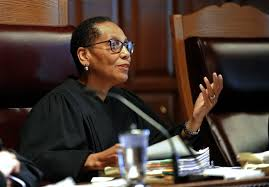
\includegraphics[width=0.3\columnwidth]{../figures/judge}};
          \uncover<2->{
            \node at (-2,-2) (jail) {
\includegraphics[width=0.3\columnwidth]{../figures/jail}};
            \draw[->] (judge) -- (jail);
          }
          \uncover<3->{
            \node at (2,-2) (bail) {
\includegraphics[width=0.3\columnwidth]{../figures/bail}};
            \draw[->] (judge) -- (bail);
          }

          \uncover<4->{
            \node at (-2,-4) (trial) {
\includegraphics[width=0.3\columnwidth]{../figures/trial}};
            \draw[->] (jail) -- (trial);
          }
          \uncover<5->{
            \draw[->] (bail) -- (trial);
          }
          \uncover<6->{
            \node at (2,-4) (arrest) {
\includegraphics[width=0.3\columnwidth]{../figures/handcuffs}};
            \draw[->] (bail) -- (arrest);
          }
        \end{tikzpicture}
      \end{column}
      \begin{column}{0.5\textwidth}
        \centering
        \uncover<7->{
          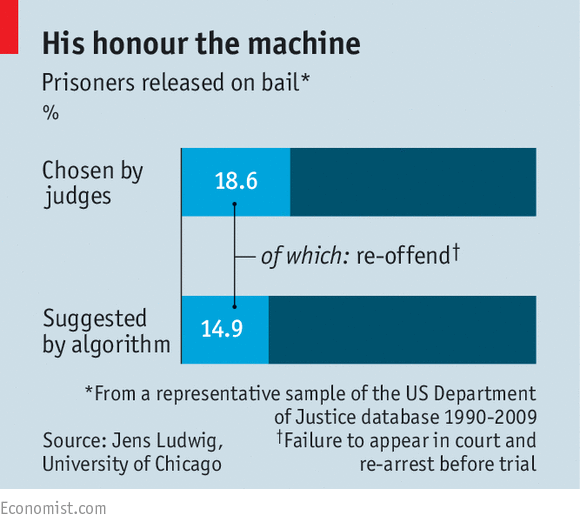
\includegraphics[width=\textwidth]{../figures/judge-fairness}
        }
      \end{column}
    \end{columns}
  }
  
  \only<article>{
    \begin{figure}
      \centering
      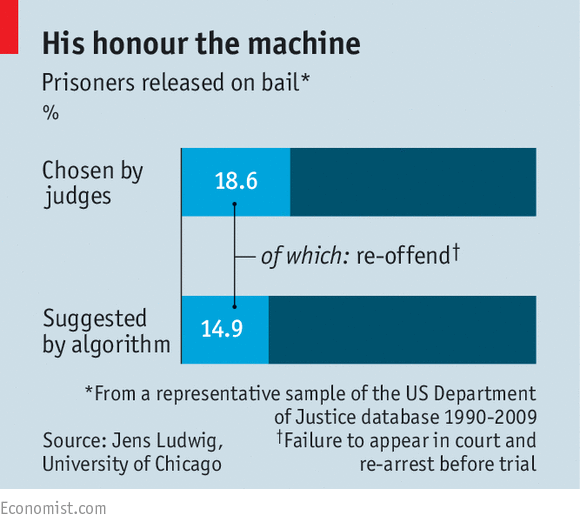
\includegraphics[width=0.5\textwidth]{../figures/judge-fairness}
      \caption{In some cases, it appears as though automating this procedure might lead to better outcomes. But is that generally true?}
      \label{fig:judge-fairness}
    \end{figure}
  }

\end{frame}

\begin{frame}
  \frametitle{Whites get lower scores than blacks\footnote{Pro-publica, 2016}}
  \only<article>{In a different study, it was shown that a commonly used software tool for determining 'risk scores' in the US was biased towards white defendants, who seemed to be always getting lower scores than blacks.}
  \begin{figure}[H]
    \begin{columns}
      \begin{column}{0.5\textwidth}
        \centering
        \def\svgwidth{0.45\textwidth}
        \input{../figures/risk-scores-black.pdf_tex}
        Black
      \end{column}
      \begin{column}{0.5\textwidth}
        \centering
        \def\svgwidth{0.45\textwidth}
        \input{../figures/risk-scores-white.pdf_tex}      
        White
      \end{column}
    \end{columns}
    \label{fig:risk-bias}
    \caption{Apparent bias in risk scores towards black versus white defendants.}
  \end{figure}
\end{frame}

\begin{frame}
  \frametitle{But scores equally accurately predict recidivsm\footnote{Washington Post, 2016}}
  \only<article>{On the other hand, the scores generated by the software seemed to be very predictive on whether or not defendants would re-offend, independently of their race.}
  \begin{figure}[H]
    \centering
    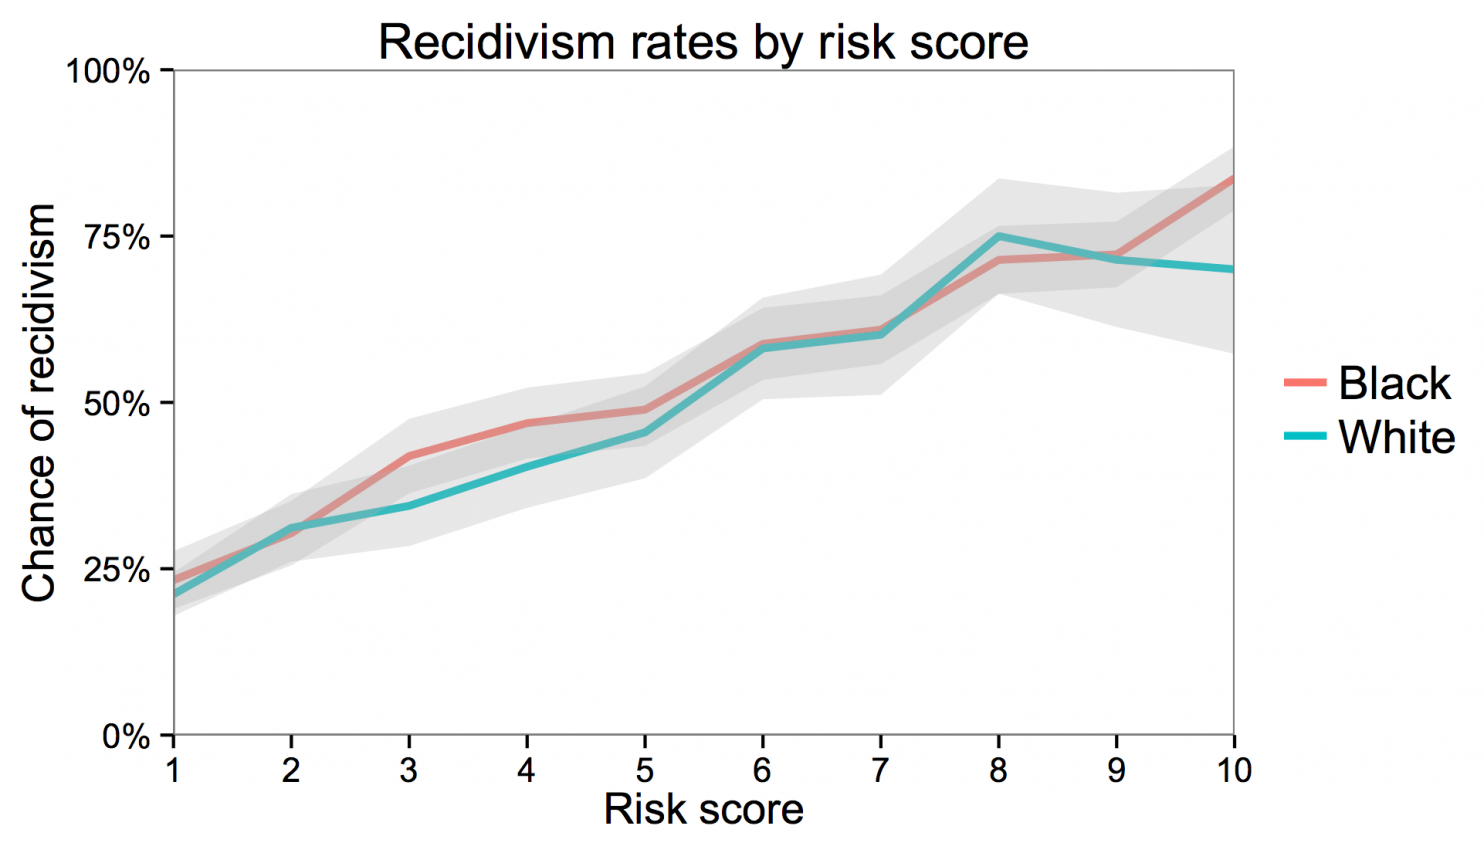
\includegraphics[width=\columnwidth]{../figures/imrs}
    \caption{Recidivism rates by risk score.}
    \label{fig:imrs}
  \end{figure}
\end{frame}
\begin{frame}
  \frametitle{But non-offending blacks get higher scores}
  \only<article>{On the third hand, we see that the system seemed to give higher risk scores to non-offending blacks. So, is there a way to fix that or not?}
  \begin{figure}[H]
    \centering
    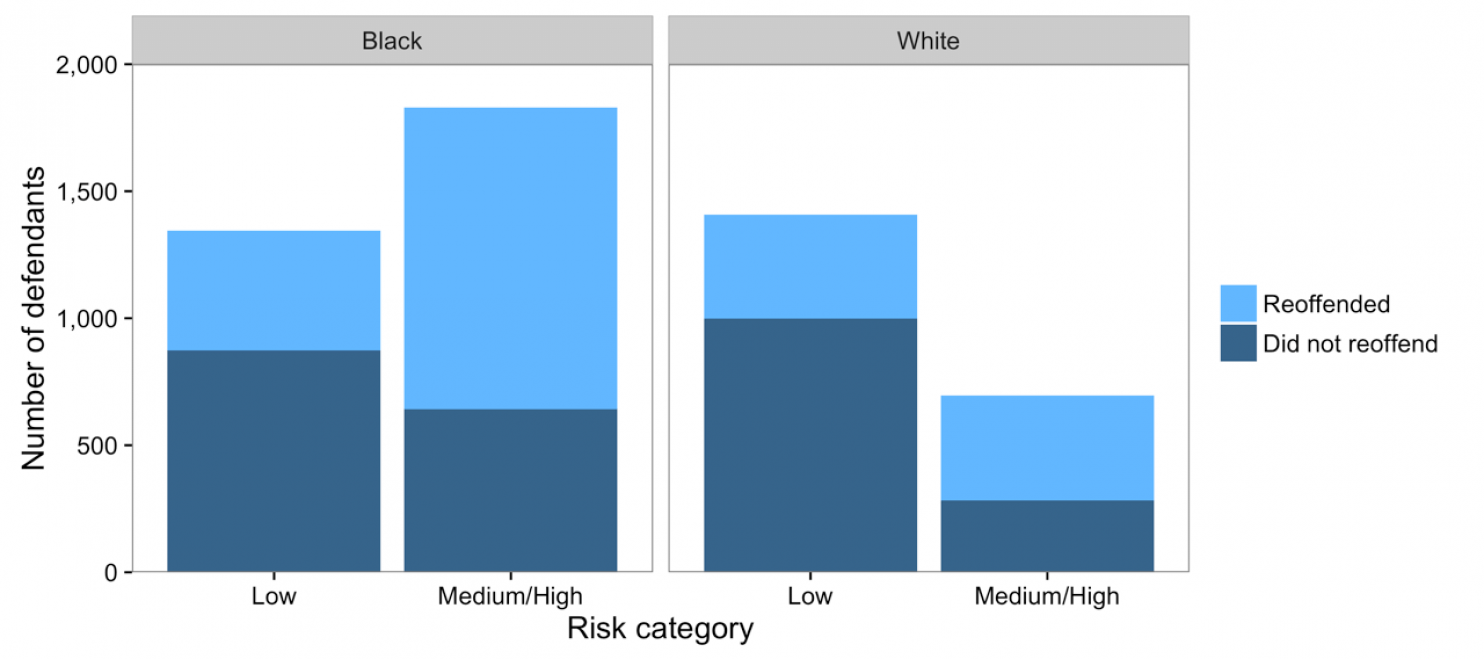
\includegraphics[width=0.5\textwidth]{../figures/imrs-risk}
    \caption{Score breakdown based on recidivism rates.}
    \label{fig:imrs-risk}
  \end{figure}
\end{frame}

\begin{frame}
  \frametitle{Bail decisions, revisited}
  \only<article>{Let us think of this problem in terms of bail decisions made by a judge using some policy $\pol$ with $\pol(a \mid x)$ being the probability that the judge decides $a$ when she observes $x$. Let $y$ be the outcome, which may or may not depend on $a$. In this particular case, $a$ is either release or jail. And $y$ is appears for trial or not. If we accept the tenets of decision theory, there is also a utility function $U(a, y)$ defined on which the judge bases her decision.}
  \only<presentation>{
    \centering

    \begin{columns}
      \begin{column}{0.5\textwidth}
        \begin{tikzpicture}
          \node[label=$x$] at (-1,2) (person)
          {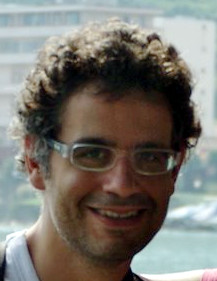
\includegraphics[width=0.2\columnwidth]{../figures/me-recent}};
          \node[label=$\pi$] at (0,0) (judge) {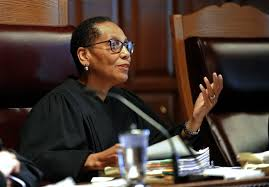
\includegraphics[width=0.3\columnwidth]{../figures/judge}};
          \draw[->] (person) -- (judge);
          \uncover<2->{
            \node[label=$a_1$] at (-2,-2) (jail) {
\includegraphics[width=0.3\columnwidth]{../figures/jail}};
            \draw[->] (judge) -- (jail);
          }
          \uncover<3->{
            \node[label=$a_2$] at (2,-2) (bail) {
\includegraphics[width=0.3\columnwidth]{../figures/bail}};
            \draw[->] (judge) -- (bail);
          }
          \uncover<4->{
            \node[label=$y_1$] at (-2,-4) (trial) {
\includegraphics[width=0.3\columnwidth]{../figures/trial}};
            \draw[->] (jail) -- (trial);
          }
          \uncover<5->{
            \draw[->] (bail) -- (trial);
          }
          \uncover<6->{
            \node[label=$y_2$] at (2,-4) (arrest) {
\includegraphics[width=0.3\columnwidth]{../figures/handcuffs}};
            \draw[->] (bail) -- (arrest);
          }
        \end{tikzpicture}
      \end{column}
      \begin{column}{0.5\textwidth}
        \uncover<2->{\[\pi(a \mid x) \tag{policy}\]}
        \uncover<4->{\[\Pr(y \mid a, x) \tag{outcome}\]}
        \uncover<7->{\[U(a,y) \tag{utility}\]}
      \end{column}
    \end{columns}
  }
  \only<article>{
    \begin{figure}[H]
      \centering
      \begin{tikzpicture}
        \node[label=$x$] at (-1,3) (person)
        {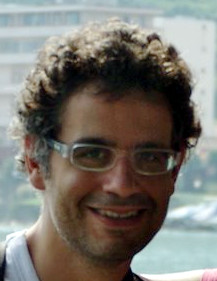
\includegraphics[width=0.1\textwidth]{../figures/me-recent}};
        \node[label=$\pi$] at (0,0) (judge) {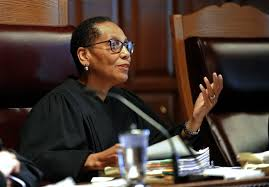
\includegraphics[width=0.2\textwidth]{../figures/judge}};
        \draw[->] (person) -- (judge);
        \uncover<2->{
          \node[label=$a_1$] at (-2,-3) (jail) {
\includegraphics[width=0.2\textwidth]{../figures/jail}};
          \draw[->] (judge) -- (jail);
        }
        \uncover<3->{
          \node[label=$a_2$] at (2,-3) (bail) {
\includegraphics[width=0.2\textwidth]{../figures/bail}};
          \draw[->] (judge) -- (bail);
        }
        \uncover<4->{
          \node[label=$y_1$] at (-2,-6) (trial) {
\includegraphics[width=0.2\textwidth]{../figures/trial}};
          \draw[->] (jail) -- (trial);
        }
        \uncover<5->{
          \draw[->] (bail) -- (trial);
        }
        \uncover<6->{
          \node[label=$y_2$] at (2,-6) (arrest) {
\includegraphics[width=0.2\textwidth]{../figures/handcuffs}};
          \draw[->] (bail) -- (arrest);
        }
      \end{tikzpicture}
      \caption{The bail decision process, simplified.}
      \label{fig:bail-process}
    \end{figure}
  }
\end{frame}


\subsection{Fairness as independence}
\begin{frame}
  \only<article>{So how can we reframe the above fairness notions in a more precise way? Both of them involve conditional independence between $y, a$ and a sensitive attribute $z$, such as race. The first notion says that the actions of the judge (or equivalently, the scores of the algorithm) are \emph{calibrated} with respect to the outcomes. The second says that they are \emph{balanced}, so that were the outcome known to the judge, she would be making a decision independently of the defendant's race.}
  \only<presentation>{
    \only<1>{
      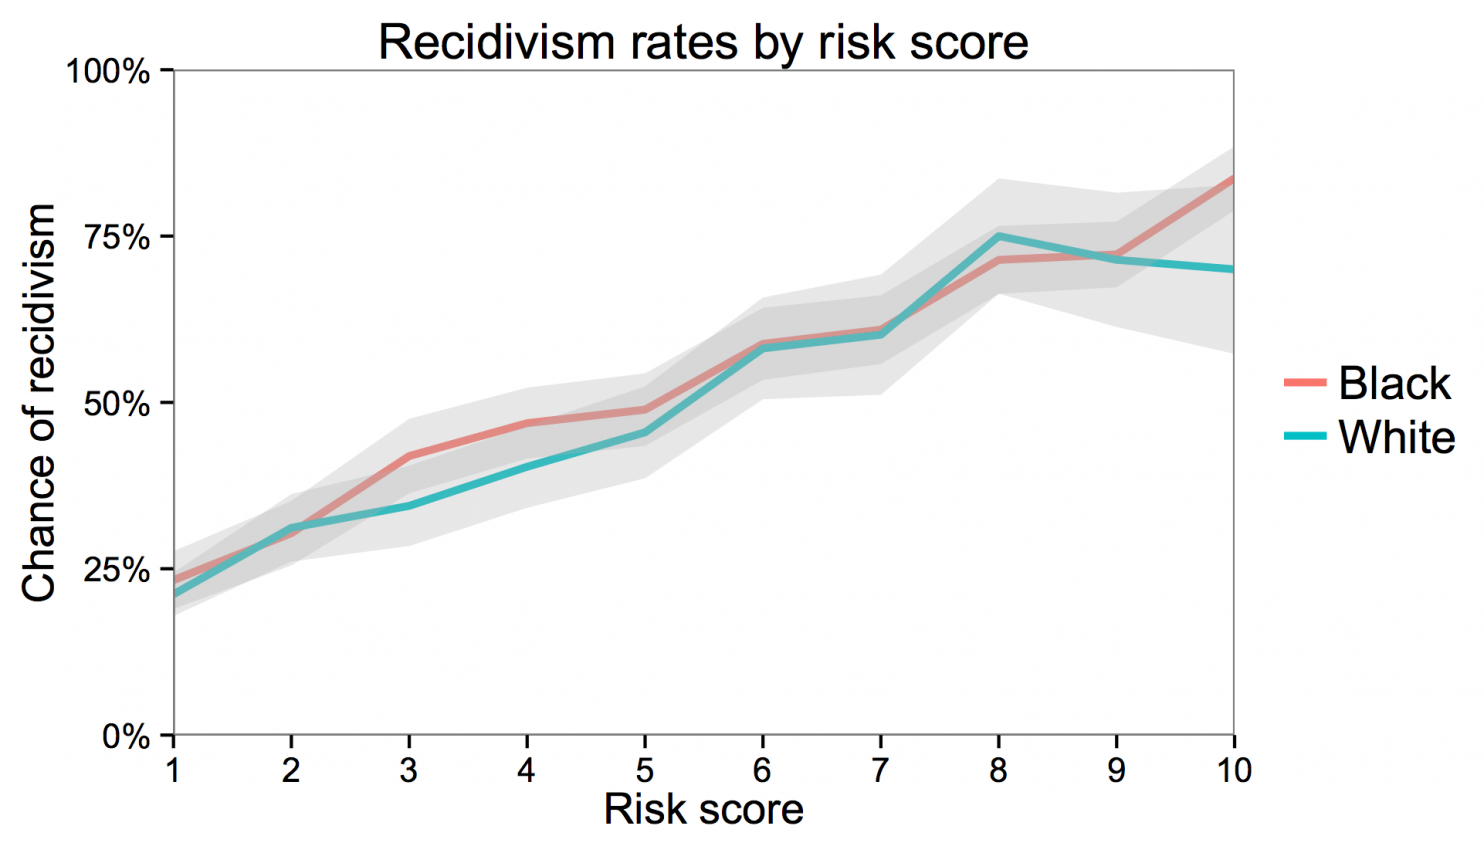
\includegraphics[width=\columnwidth]{../figures/imrs}
    }
    \only<2>{
      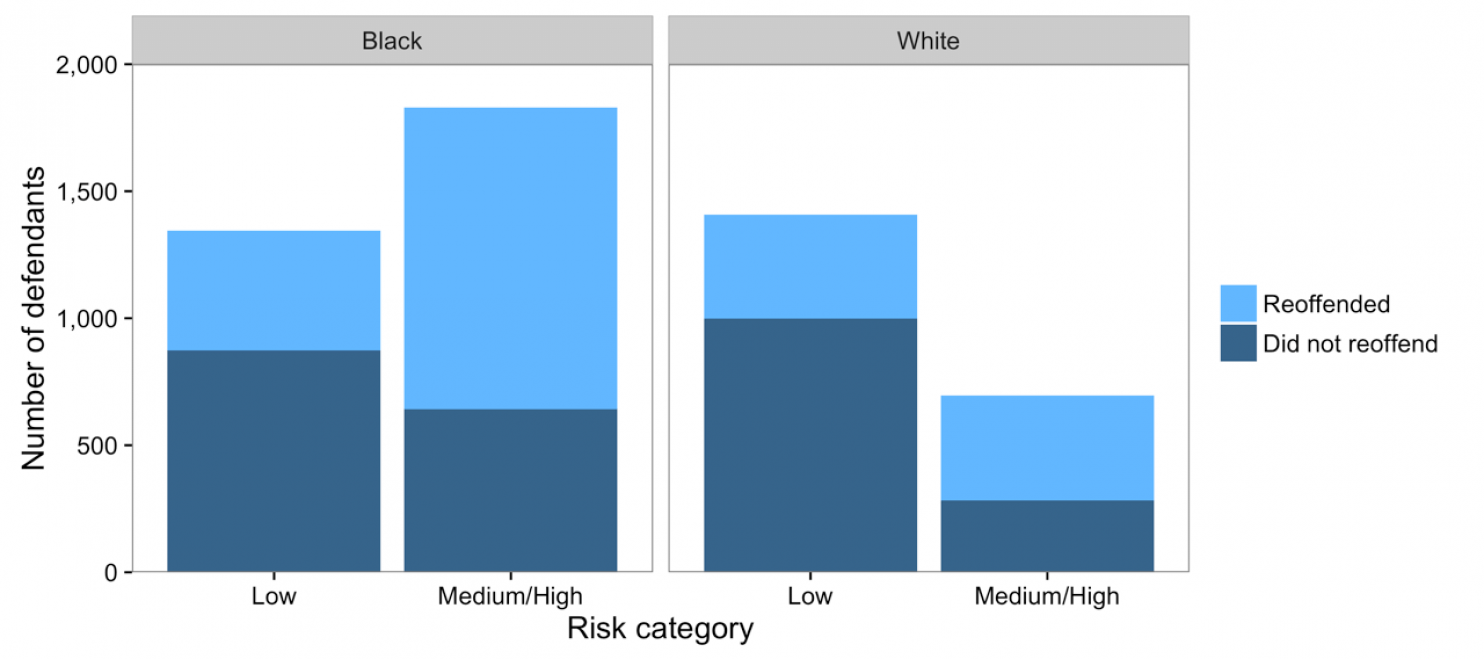
\includegraphics[width=\columnwidth]{../figures/imrs-risk}
    }
    \begin{columns}
      \begin{column}{0.3\textwidth}
        \begin{itemize}
        \item[$y$] Result.
        \item[$a$] Assigned score.
        \item[$z$] Race.
        \end{itemize}
      \end{column}
      \begin{column}{0.7\textwidth}
        \begin{align}
          \Pr^\pi(y \mid a, z) &= \Pr^\pi(y \mid a) \tag{\alert<1>{calibration}}\\
          \Pr^{\pi}(a \mid y, z) &= \Pr^{\pi}(a \mid y) \tag{\alert<2>{balance}}
        \end{align}
      \end{column}
    \end{columns}
  }
  \only<article>{
    \begin{definition}[Calibration]
      A policy $\pol$ is calibrated for parameter $\param$ with respect to $z$ if
      \begin{equation}
        \Pr_\param^\pol(y \mid a, z) = \Pr_\param^\pol(y \mid a), \qquad \forall a, z.
        \label{eq:calibration}
      \end{equation}
    \end{definition}
    You will observe that calibration here means that
    \[
      y \indep z \mid a, \param, \pol
    \]
    i.e. that $y$ is independent of $z$ given the judge's action $a$, so the distribution of outcomes is the same for every one of our actions no matter what the value of $z$ is.

    \begin{definition}[Balance]
      A policy $\pol$ is balanced for parameter $\param$ with respect to $z$ if
      \begin{equation}
        \Pr_\param^{\pol}(a \mid y, z) = \Pr_\param^{\pol}(a \mid y), \qquad \forall y, z.
        \label{eq:balance}
    \end{equation}
    \end{definition}
    On the other hand, balance means that
    \[
      a \indep z \mid y,
    \]
    i.e. that $a$ is independent of $z$ given the true outcome $y$.\footnote{This definition only really makes sense when $y$ does not depend on $a$ at all. When this is not the case, it's easy to construct a random variable $y'$ that does not depend on $a$ so that $y$ can be written as a function $y(y', a)$. Then we can achieve balance with respect to $y'$.}
  }

  \only<article>{In both cases, we defined conditional independence for a fixed probability distribution $P_\param(x,y,z)$ on the various variables.}
\end{frame}

\subsection{Fairness as meritocracy.}
  \only<article>{A different concept of fairness is meritocracy. For example, if one candidate for a job is better than another, shouldn't that candidate be always preferred? How can we formalise this?}


\begin{frame}

  \only<article>{Let us consider merit from the point of view of the decision maker, who can either hire $(a_t = 1)$ or not hire $(a_t = 0)$ the $t$-th applicant. If the applicant has characteristics $x_t$ and merit $y_t$, the DM's decision has utility $U(a_t, y_t)$. In order to model meritocracy, we assign an inherent \emph{quality} to $y$, expressed as an ordering, so that $U(1, y) \geq U(1, y')$ if $y \geq y'$. Assuming $P_\param(x_t, y_t)$ is known to the DM then clearly she should make the decision by solving the following maximisation problem:
  }
  \begin{align}
    a_t(\param, x_t) \in \argmax_a \E_\param(U \mid a, x_t)
    &=
      \int_\CY U(a_t, y) \E_\param(U \mid a_t, x_t) 
  \end{align}
  
  \only<article>{
    Here, the notion of meritocracy is defined through our utility function. The expectation here is essentially taken because we may not know for certain what the quality attribute of a given person might be.
  }
\end{frame}
\subsection{Fairness as similarity.}
\begin{frame}
  \only<article>{It makes sense to combine the idea of meritocracy with that of similarity. That is, similar people should be treated similarly. This means that we should find a policy $\pol$ that maximises utility $\util$ and makes similar decisions for similar people. We can formalize this as}
  \[
  D(\pol(a \mid x), \pol(a \mid x')
  \leq 
  \rho(x, x').
  \]
  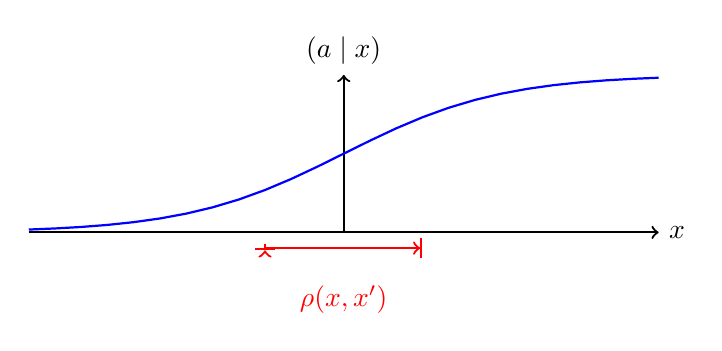
\begin{tikzpicture}[scale=2,thick,domain=-2:2]
    \draw[->] (-2,0) -- (2,0) node[right] {$x$};
    \draw[->] (0,0) -- (0,1) node[above] {$\pol(a \mid x)$};
    \draw[color=blue] plot (\x,{0.5 + 0.5 * tanh(\x)}); % node[right] {$f(x) = \frac{1}{20} \mathrm e^x$};
    \draw [|<->|,color=red] plot (-0.5,-0.1) -- node[below=1em] {$\rho(x,x')$} ++(1, 0);
  \end{tikzpicture}
\end{frame}








%%% Local Variables:
%%% mode: latex
%%% TeX-engine: xetex
%%% TeX-master: "notes"
%%% End:
